\documentclass{article}
\usepackage[utf8]{inputenc}
\usepackage[francais]{babel}
\usepackage{lmodern}
\usepackage[a4paper, margin=3cm]{geometry}
\usepackage{fancyhdr}

%Package for math expression
\usepackage{amsmath}
\usepackage{cancel}
\usepackage{amsthm,amstext,amsfonts,bm,amssymb,amsthm}
\usepackage{bm}
\usepackage{gensymb}
\usepackage{mathrsfs}
\usepackage{physics}
\usepackage{nicefrac}
\usepackage{pgffor}

%Package for graphic expression
\usepackage{graphicx}
\usepackage{wrapfig}
\usepackage{float}
\usepackage{caption}
\usepackage{subcaption}
\usepackage{enumitem}
\usepackage{fancyhdr}
\usepackage{sectsty}
\usepackage{multirow}

\usepackage{mathtools}
\DeclarePairedDelimiter\ceil{\lceil}{\rceil}
\DeclarePairedDelimiter\floor{\lfloor}{\rfloor}

\usepackage{pgffor}

\DeclarePairedDelimiter\absol{\lvert}{\rvert}%

% Header
\pagestyle{fancy}
\fancyhf{}
\rhead{Éric Pfleiderer}
\fancyhead[L]{Algorithmes évolutifs: l'orbite de $\rho$CrB}
\chead{}
\rfoot{}
\cfoot{\thepage}

\begin{document}
	
\begin{titlepage}
	\centering
	\vspace*{1cm}
	\textsc{\LARGE Université de Montréal}\\[1cm] 
	\textsc{\Large PHY 3075 -- Modélisation Numérique en Physique}\\[3cm]
	\vspace{1cm}
	\rule{\linewidth}{0.5mm} \\[0.5cm]
	{\LARGE \bfseries Algorithmes évolutifs: \\ l'orbite de $\rho$CrB} \\[0.2cm]
	\rule{\linewidth}{0.5mm} \\[3cm]
	\vspace{1cm}
	\large par: \\*
	Éric Pfleiderer \\* 
	20048976\\[3cm] 
	\vspace{1cm}
	{\large \today}\\[3cm]
	\vfill
\end{titlepage}

\section*{Résumé}\label{sec:resume}

L'objectif de ce laboratoire est l'exploration des algorithmes évolutifs et de leurs applications sous deux contextes: la diffraction en deux dimensions et l'optimisation d'un modèle d'orbite képlérienne à $6$ paramètres à partir d'observations de vitesse radiales. Le premier contexte sert à faciliter la visualisation de l'espace paramétrique et à valider l'algorithme. Ensuite, on explore l'influence de $4$ hyperparamètres, $N$, $p_c$, $p_m$ et $p_s$, sur les solutions produites par l'algorithme. Additionnellement, on explore $3$ types de mutations adaptives: basées sur l'objectif, basées sur la distance et non-uniformes. Ces méthodes adaptives sont mises en compétition pour déterminer le type de mutations employées lors de l'optimisation finale des données. On trouve que la performance des stratégies est comparable à l'exception de la stratégie basée sur la distance. La méthode choisie pour l'optimisation du modèle est celle basée sur l'objectif, qui demeure plus stable lorsqu'on considère l'ensemble des solutions produites. On suggère le vecteur solution final $v^f_{sol} = (39.80\pm0.04, 85\pm50, 2.1\pm0.4, 0.110\pm0.005, 63.9\pm0.6, -47\pm1)$ pour l'ensemble de paramètres $P$, $\tau$, $\omega$, $e$, $K$, et $V_0$.

\section{Introduction}\label{sec:introduction}

Une quête perpétuelle de l'analyse numérique est sans doute le problème de l'optimisation. Plus spécifiquement, comment peut-on éviter de converger vers un minimum local lors d'un ajustement de données? Existe-t-il des techniques pour augmenter la probabilité de converger vers un maximum global? Peut-on s'inspirer de phénomènes biologiques pour développer des algorithmes dotés de comportements complexes? La pertinence de ces questions prend de l'importance avec la popularité grandissante des réseaux neuronaux qui basent leur entraînement sur de telles techniques.

L'objectif de ce laboratoire est donc l'exploration des algorithmes évolutifs et des techniques de mutations adaptives. On applique d'abord un algorithme évolutif sur un problème de diffraction à deux dimensions afin de faciliter la visualisation de données et la validation des résultats. On s'intéresse ensuite au contexte d'application principal, soit l'ajustement d'un modèle d'orbite képlérienne aux systèmes binaires $\rho Corona Borealis$ et $\eta Bootis$. On emploie initialement des mutations de tailles constantes et on étudie l'influence des hyperparamètres  $N$, $p_m$, $p_c$ et $p_c$ sur la convergence. On introduit ensuite $3$ types de stratégies de mutations adaptives; basée sur l'objectif, basée sur la distance paramétrique et non-uniforme. Les différentes méthodes sont mises en compétition pour déterminer laquelle est la plus prometteuse. Finalement, on procède à la tâche principale; l'optimisation des paramètres du modèle à l'aide de données décrivant le système $\rho Corona Borealis$.

\section{Théorie}\label{sec:theorie}

\subsection{La diffraction}

La diffraction décrit le comportement d'une onde lorsqu'elle rencontre une ouverture. Elle est expliquée par le principe de Huygens-Fresnel, qui suppose que chaque point d'un front d'onde se comporte comme une collection d'ondes. On introduit l'équation \ref{eq:diffraction}, qui définit la relation entre l'intensité normalisée d'une onde et sa position en deux dimensions. La figure \ref{fig:diffraction}, quant à elle, affiche un patron de diffraction en 1 et en 2 dimensions spatiales. L'intensité est normalisée de sorte que $I_{max}=1$ à l'origine.

\begin{equation}\label{eq:diffraction}
	\frac{I(x,y)}{I_0} = \left(\frac{sin(x)}{x}\frac{sin(y)}{y}\right)^2
\end{equation}

On estime l'erreur d'une certaine solution $v_{sol}=(x, y)$ par l'équation \ref{eq:diff_erreur}, qui est simplement une différence entre le maximum global à l'origine et la valeur de notre solution.

\begin{equation}\label{eq:diff_erreur}
e = I_{max} - I(v_{sol}) = 1 - I(v_{sol})
\end{equation}

La recherche du maximum global est compliquée par la présence de plusieurs maxima locaux dus aux termes sinusoïdaux dans l'équation \ref{eq:diffraction}. L'équation de diffraction exhibe une des vulnérabilités de la descente du gradiant traditionnelle, qui converge vers l'extremum local le plus près du point de départ. Il s'agit de conditions idéales à l'application des algorithmes évolutifs.

\subsection{L'orbite képlérienne}

La méthode principale d'identification des système binaires est par étude du décalage Doppler causé par le mouvement orbital.
Ce mouvement orbital est décrit par l'équation \ref{eq:V}, où $V$ est la vitesse radiale observée, $K$ est l'amplitude de vitesse, $e$ est l'excentricité de l'orbite et $\omega$ est le déphasage. 

\begin{equation}\label{eq:V}
	V(t) = V_0 + K[cos(w+v(t)) + e\ cos(\omega)]
\end{equation}

L'anomalie de la vitesse projetée $v$ est obtenue à l'aide de la relation \ref{eq:E}, où $E$ est l'anomalie excentrique. 

\begin{equation}\label{eq:v}
	tan \left(\frac{v}{2}\right) - \sqrt{\frac{1+e}{1-e}}\ tan\left(\frac{E}{2}\right) = 0
\end{equation}

Finalement, l'anomalie $E$ est reliée au temps $t$ par l'équation de Kepler (voir équation \ref{eq:E}), où $P$ est la période et $\tau$ est le temps de passage au périhélion. L'équation de Kepler définit un problème de recherche de racine non-linéaire, qu'on résoud par bissection.

\begin{equation}\label{eq:E}
	E - e\ sin(E) - \frac{2 \pi}{P}(t - \tau)=0 
\end{equation}

Ensemble, les paramètres $P, \tau, \omega, e, K$ et $V_0$ définissent un espace paramétrique à 6 dimensions. C'est cet espace, 
où chaque point peut être décrit par un vecteur solution $v_{sol} = (P, \tau, \omega, e, K, V_0)$, que l'algorithme évolutif tente d'explorer.

\section{Méthodologie}\label{sec:methodologie}


\subsection{Analyse numérique}\label{subsec:analyse_numerique}

Les algorithmes évolutifs sont des procédés itératifs et stochastiques qui sont souvent inspirés de la génétique. Ils possèdent généralement les phases suivantes; l'initialisation, l'évaluation, le classement, la sélection, la reproduction et le remplacement. On introduit ici la notion d'hyperparamètre; un paramètre qui concerne l'algorithme plutôt que le modèle d'orbite képlérienne. Ces hyperparamètres en questions, $N$, $p_c$, $p_m$ et $p_s$, sont introduits dans les prochaines sections. Leur objectif est de contrôler le comportement de la population. L'implémentation particulière de l'algorithme employée durant ce laboratoire est disponible sur le repos GitHub de l'auteur\cite{github}.

\vspace{0.3cm}
\noindent\textbf{Initialisation}

La première étape consiste à définir une populations de plusieurs vecteurs solutions $v_{sol}$ initiaux qui déterminent les points de départ de l'algorithme. Un choix judicieux de chaque $v_{sol}$ demeure important et peut être informé par la définition des paramètres et par une étude des données. Les intervalles choisis et employés sont affichés au tableau \ref{tab:intervalles}.

\begin{table}[H]
	\begin{center}
		\caption{Intervalle pour chaque paramètre à optmiser. Les paramètres sont initialisés et contraints à ces intervalles durant l'optimisation.}
		\label{tab:intervalles}
		\begin{tabular}{c|c|c} % <-- Changed to S here.
			\textbf{paramètre} & \textbf{intervalle} & \textbf{unités}\\
			\hline	
			\hline
			$P$ & $200 \le P \le 800 $ & $J.D.$\\
			$\tau$ & $t_0 \le \tau \le t_0 + P$ & $J.D.$\\
			$\omega$ & $0 \le \omega \le 2 \pi$ & $radian$\\
			$e$ & $0 \le e \le 1$ & $[1]$\\
			$K$ & $0 \le K \le max(V_j)-min(V_j)$ & $km\ s^{-1}$\\
			$V_0$ & $min(V_j) \le V_0 \le max(V_j)$ & $km\ s^{-1}$\\
		\end{tabular}
	\end{center}
\end{table}

\vspace{0.3cm}
\noindent\textbf{Évaluation}

La deuxième phase consiste à définir une fonction objectif pour guider notre recherche, c'est-à-dire qui décrit la qualité d'un vecteur solution. On utilise les données fournises\cite{diro} pour calculer un khi-deux, définit par l'équation \ref{eq:khi_deux}, qu'on minimise en réduisant l'écart entre les observations et les prédictions. Puisque notre algorithme s'applique sur des problèmes de maximisation, on s'intéresse plutôt à l'inverse du khi-deux, qui définit notre fonction objectif (voir équation \ref{eq:fonction_obj}). 

\begin{equation}\label{eq:khi_deux}
	\chi^2(v_{sol}) = \frac{1}{N-6} \sum_{i=0}^{N} \left(\frac{V_{i}^{obs} - V(v_{sol}, t_i)}{\sigma_i})\right)^2
\end{equation}

\begin{equation}\label{eq:fonction_obj}
	f_{obj}(v_{sol}) = \frac{1}{\chi^2(v_{sol})}
\end{equation}

Lorsque la différence entre les observations et les prédictions sont similaires en grandeur à l'erreur associé aux mesures, on termine l'algorithme afin d'éviter la suroptimisation; le modèle ne doit pas incorporer les déviations dues aux erreurs, mais plutôt le comportement général des données.

\vspace{0.3cm}
\noindent\textbf{Classement et sélection}

Lorsque chaque individu est évalué, on procède ensuite au classement et à la sélection. Le classement consiste ici simplement à hiérarchisé les solutions à l'aide de $f_{obj}$. La sélection est effectuée par le biais d'un paramètre de pression sélective $p_s \in [0, 1]$ qui décrit la probabilité que chaque membre de la population soit choisit pour la reproduction.  Une valeur nulle se traduit par un absence de biais, tandis qu'une valeur de 1 implique que seul la meilleur solution courante est reproduite.

\vspace{0.3cm}
\noindent\textbf{Reproduction}

Une fois les parents choisis, ils ont une probabilité $p_m$ de se reproduire.  S'ils échouent à la reproduction, on observe une reproduction asexuée de chaque parent; les enfants sont des clones identiques. Par contre, s'ils se reproduisent avec succès, il y a \textit{échange du matériel génétique}. Étant donnée deux parents $p_1$ et $p_2$, on déduit le paramètre $i$ de deux enfants $c_1$ et $c_2$ par combinaison linéaire (voir équation \ref{eq:reprod}).

\begin{equation}\label{eq:reprod}
	\begin{gathered}
		i_{c_1} = ai_{p_1} + (1-a) i_{p_2}\\
		i_{c_2} = (1-a)i_{p_1} + a i_{p_2}\\
		a\ \sim U(0, 1)
	\end{gathered}
\end{equation}

Lors de la reproduction, les enfants générés ont une probabilité $p_c$ de subir une mutation aléatoire. Les types de mutations prennent plusieurs forment et sont explicités à la section \ref{sec:mutations_adaptives}. Puisque les paramètres à optimiser ne sont pas tous de la même ordre de grandeur, on définit un vecteur de mutation $v_{mut}$, qui définit la taille de pas associé à chaque composante du vecteur solution $v_{sol}$. Le vecteur $v_{mut}$ est initialisé en moyennant la valeur de chaque paramètre à travers la population et en choisissant une certaine proportion de cette quantité.


\begin{equation}\label{mutation_ini}
	v_{mut} = c \overline{v}_{sol},\ c\ \in\ \real
\end{equation}

La mutation non adaptive employée dans les premières sections du laboratoire est définie par l'équation \ref{eq:mutation}, où $v^i_{mut}$ est la $i^e$ composante du vecteur de mutation. 

\begin{equation}\label{eq:mutation}
	c^{n+1}_{i} = c^{n}_{i} + G(0, \absol{v^i_{mut}})
\end{equation}

\vspace{0.3cm}
\noindent\textbf{Remplacement}

Finalement, il ne reste plus qu'à remplacer la génération précédente par les enfants et continuer à itérer. Par contre, une technique essentielle doit être implémentée: l'élitisme. On préserve artificiellement la meilleur solution à chaque étape, ce qui nous garanti de ne jamais rétrograder durant l'exploration de l'espace paramétrique. 


\section{Résultats}\label{sec:resultat}

\subsection{Validation des résultats}

On s'intéresse d'abord à explorer le comportement de notre algorithme évolutif dans un contexte où la visualisation et l'exploration de l'espace paramétrique est facilitée: la diffraction en deux dimensions. On définit un intervalle d'étude de $X \times Y,\ X,Y \in [-2 \pi, 2 \pi]$ et on initialise une population de $N=10$ individus distribués uniformément dans ce domaine. On applique les processus itératifs décrits à la section \ref{sec:methodologie} en évaluant la qualité des solutions à l'aide de l'équation \ref{eq:diffraction}. La figure \ref{fig:diffraction_instant} affiche les instantannées de la simulation pour les 9 premières étapes. Le point vert représente la solution optimale à chaque étape, tandis que la courbe verte affiche la trajectoire de la solution optimale de génération en génération. On remarque que l'initialisation aléatoire des positions place la solution optimale très près d'un maximum local, ce qui serait une situation facheuse si on utilisait la descente du gradient traditionnelle. Dans notre cas, une mutation ou un croisement déplace la solution optimale près d'un second maximum local qui s'avère supérieur au précédent. L'algorithme demeure sur cet extremum jusqu'à l'étape 4, où il débute enfin à grimper le maximum global. À ce point, l'élitisme nous garantit de ne pas régrésser; la convergence continue indéfiniment jusqu'à ce que l'erreur \ref{eq:diff_erreur} devienne plus petite que l'epsilon de la machine employée. La figure \ref{fig:diffraction_error} affiche l'erreur correspondant à la simulation de la figure \ref{fig:diffraction_instant} ainsi que l'erreur d'une simulation de $100$ générations. 

Une fois assuré de la validité de notre algorithme, on cherche à implémenter une seconde version sur le sujet central du laboratoire, soit l'ajustement d'un modèle képlérien décrivant les orbites de $\eta Bootis$ et $\rho CoronaBorealis$. On s'intéresse d'abord à $\eta Bootis$, pour lequel un vecteur solution $v_{sol} = (494.20, 14299.0, 5.7397, 0.2626, 8.3836, 1.0026)$ est fourni \cite{notes_cours}. Dans le cas présent, l'espace paramétrique est de 6 dimensions et est difficile à visualiser. On offre plutôt la figure \ref{fig:convergence_orbite}, qui montre les observations ainsi que le modèle ajusté pour 3 étapes de la simulations, soit à 100, 250 et 500 générations. On observe bien la convergence désirée; le modèle se juxtapose aux données et converge vers la solution fournise. On entame alors la tâche d'étudier l'impact des hyperparamètres sur le comportement de l'algorithme.

\subsection{Influence des hyperparamètres}

L'implémentation de l'algorithme évolutif permet la manipulation de $4$ hyperparamètres, soit $N$, $p_m$, $p_c$ et $p_s$. Ces paramètres contrôlent et influence l'exploration de l'espace paramétrique ainsi que le rythme de convergence. Par exemple, on sait qu'une augmentation de la population $N$ entraîne une exploration additionnelle de l'espace paramétrique pour chaque nouvel individu. On s'attend donc à ce que la taille de la population impacte la capacité de l'algorithme à trouver le maximum global. Ensuite, par analogie à la génétique, l'information de population est partagée par reproduction sexuée entre ses membres. L'introduction d'une nouvelle information génétique provient des mutations. On s'attend donc à ce que le facteur $p_m$ influence l'exploration en définissant la fréquence d'introduction de nouvelle information. Ensuite, $p_c$ caractérise la popularité de la reproduction séxuée et asexuée. On s'attend à ce qu'un haut taux de reproduction augmente la convergence vers la solution optimale courante. Finalement, la pression de sélection $p_s$ détermine quels individus sont considérés durant la phase de reproduction. On s'attend à ce qu'une pression trop élevée cause une convergence prématurée vers une solution sous optimale, tandis qu'une pression trop faible diminue la capacité de convergence dans les phases terminales de la simulation.

On compare nos prédictions avec la figure \ref{fig:parametres}, qui montre l'influence de chaque paramètre sur la solution finale. On contrôle la génération stochastique des nombres afin de diminuer la dépendance sur la solution initiale. On remarque, tel que prédit, qu'une augmentation de la taille de la population mène habituellement à une meilleur solution. Ensuite, on constate que l'hyperparamètre $p_m$ doit être restreint à des valeurs $<<1$. Lorsque $p_m \approx 1$, le $\chi^2$ tend à demeurer constant jusqu'à subir une diminution importante et subite; l'algorithme est incapable de converger vers l'extremum le plus près de la solution optimale courante et tend à optimiser la fonction objective en trouvant un extremum de meilleure qualité. C'est un comportement recherché en début de simulation, mais lorsque celle-ci mature, on assume que le maximum global est repéré et on désire plutôt imposer un biais pour l'affinement de la solution courante. Quant à $p_s$, on remarque que nos prédictions sont supportées par cette simulation; on cherche un compromis entre l'exploration par le hasard et la convergence par sélection sévère. Finalement, la probabilité d'accouplement $p_c$ n'influence pas significativement la capacité de convergence dans cet exemple. Tôt ou tard, on atteint le même extremum. 


\subsection{Les mutations adaptives}\label{sec:mutations_adaptives}

On s'intéresse maintenant à implémenter plusieurs stratégies de mutations adaptives; on tente d'améliorer la performance de notre aglorithme et on cherche à comparer les différentes stratégies entres-elles. On introduit $3$ types de mutations adaptives, soit la mutation basée sur la fonction objectif, la mutation basée sur la distance et la mutation non-uniforme.

\vspace{0.3cm}
\noindent\textbf{Basé sur la fonction objectif}

Le vecteur de mutation $v_{mut}$ est potentiellement modifié à chaque génération par multiplication ou division par un scalaire $c$. La décision de modifier $v_{mut}$ est effectuée à partir d'une différence entre la valeur de l'objectif de la  solution optimale courante $v^1_{sol}$ et celle de la solution médiane $v^{med}_{sol}$. Si la différence est plus petite qu'une fraction $a$ de $v^1_{sol}$, on assume que la convergence est trop forte; on augmente le pas. Par contre, si la différence est plus grande qu'une fraction $b$ de $v^1_{sol}$, on assume que la population possède une bonne étendue paramétrique et on diminue la taille du pas afin de faciliter la convergence locale.

\begin{equation}
	v^{n+1}_{mut} = \begin{cases}
						cv^{n}_{mut}, & si\ f(v^1_{sol}) - f(v^{med}_{sol}) \le a f(v^1_{sol}),\ a,c\ \in\ \real \\
						\frac{v^{n}_{mut}}{c}, & si\ f(v^1_{sol}) - f(v^{med}_{sol}) \ge bf(v^1_{sol}),\ b,c\ \in\ \real
					\end{cases}  
\end{equation}

\vspace{0.3cm}
\noindent\textbf{Basé sur la distance}

Le vecteur de mutation $v_{mut}$ est potentiellement modifié à chaque génération par multiplication ou division par un scalaire $g(c)$ provenant d'une distribution gaussienne $G$. La décision de modification est basée sur la distance paramétrique entre $v^1_{sol}$ et la $v^{med}_{sol}$. Si la distance est plus petite que $a$, on assume que la population est trop concentrée dans l'espace paramétrique et on augmente la taille de $v_{mut}$. Au contraire, Si la distance est plus grande que $b$, on réduit $v_{mut}$.

\begin{equation}
	v^{n+1}_{mut} = \begin{cases}
						g(c)\ v^{n}_{mut},\ g(c)\ \sim\ G(1+3c, c), & si\ \norm{v^1_{sol} - v^{med}_{sol}} \le a,c\ \in\ \real\\
						\frac{v^{n}_{mut}}{g(c)},\ g(c)\ \sim\ G(1+3c, c), & si\  \norm{v^1_{sol} - v^{med}_{sol}} \ge b,c\ \in\ \real \\
					\end{cases}  
\end{equation}

\vspace{0.3cm}
\noindent\textbf{Non-uniforme}

Dans le cas des mutations non-uniformes, le vecteur $v_{sol}$ est modifié directement au lieu d'employer $v_{mut}$. Cette méthode\cite{neurodim} réduit graduellement l'amplitude des mutations avec chaque nouvelle génération; on tente d'imposer un biais d'exploration au début de la simulation et un biais de convergence vers la fin. À chaque génération, on ajoute à chaque composante de $v_{sol}$ une contribution provenant d'une distribution gaussienne centrée en $0$. Un variable binomiale $l$ détermine si on somme ou soustrait cette contribution. L'écart type est définit par l'équation \ref{eq:delta}, où le premier terme est l'écart entre une composante et une borne, $r$ est une variable suivant une distribution uniforme et le troisième terme est responsable de supprimer l'amplitude des mutations lorsque la simulation mature. Le terme $b$ contrôle à quel rythme les mutations sont supprimées et détermine donc fortement le biais imposé entre l'exploration et convergence. 

\begin{equation}\label{eq:nu}
	v^{n+1}_{sol} = \begin{cases}
					v^{n}_{sol} + G(0, \absol{\Delta_1}) & si\ l=0,\ l \sim B(p=0.5)\\
					v^{n}_{sol} - G(0, \absol{\Delta_2}) & si\ l=1,\ l \sim B(p=0.5)\\
					\end{cases}  
\end{equation}

\begin{equation}\label{eq:delta}
	\begin{gathered}
		\Delta_1  = (v_{max} - v_{sol})\ r\ \left(1-\frac{t}{t_{max}}\right)^c,\ r\ \sim\ U(a,b),\ a,b,c\ \in\ \real \\
		\Delta_2  = (v_{sol} - v_{min})\ r\ \left(1-\frac{t}{t_{max}}\right)^c,\ r\ \sim\ U(a,b),\ a,b,c\ \in\ \real
	\end{gathered}
\end{equation}


\vspace{0.3cm}
\noindent\textbf{Comparaison de performance}

Dans le but de sélectionner la meilleure stratégie, on organise une compétition entre les types de mutations, incluant la stratégie non adaptive qu'on nomme standard. Chaque scénario implique $25$ simulations de $1000$ générations. On liste un sommaire de la compétition au tableau \ref{tab:competition}. On remarque rapidement que les solutions offertes par les différentes stratégies sont toutes similaire, sauf pour celle basée sur la distance. L'implémentation de cette méthode converge avec difficulté; on l'élimine des candidats pour l'optimisation. Ensuite, on constate que les pires solutions offertes sont aussi très similaires, sauf dans le cas de la fonction objectif, qui offre une solution inférieure d'une ordre de grandeur. Par contre, il est difficile d'évaluer si cette différence est due à la nature stochastique de l'algorithme ou à la méthode de mutation. Finalement, on s'intéresse à la synthèse des résultats. Parmis les trois stratégies restantes, les meilleurs solutions sont pratiquement homogènes. Par contre, la stratégie des mutations basées sur la fonction objectif se démarque des autres par sa faible moyenne sur l'ensemble des résultats. Sous ces considérations, on choisit de progresser avec cette méthode.


\begin{table}[H]
	\begin{center}
		\caption{Résultats d'une compétition entre les types de mutations. Les simulations comptent $N=10$ individus, une pression sélective $P_s=0.25$, une probabilité de croisement $P_c=0.8$ et une probabilité de mutation $P_m=0.1$. On lance $25$ simulations de $1000$ générations pour chaque type de mutation et on affiche la valeur du khi-deux pour les $5$ meilleurs solutions et pour la pire. On affiche additionnellement la moyenne et l'écart type pour les $5$ meilleurs solutions, ainsi que pour l'ensemble des résultats.}
		\label{tab:competition}
		\begin{tabular}{|c|c|c|c|c|} % <-- Changed to S here.
			\hline	
			\textbf{$\chi^2$} & \textbf{Standard} & \textbf{Objectif} & \textbf{Distance} & \textbf{Non-Uniforme}\\\hline\hline
			$\chi_1^2$ & $0.36642$ & $0.36559$ & $0.53122$ & $0.36615$\\
			$\chi_2^2$ & $0.36677$ & $0.36591$ & $0.57684$ & $0.36671$\\
			$\chi_3^2$ & $0.36765$ & $0.36594$ & $0.59317$ & $0.36700$\\
			$\chi_4^2$ & $0.37007$ & $0.36600$ & $0.62379$ & $0.36879$\\
			$\chi_5^2$ & $0.37139$ & $0.36622$ & $0.69896$ & $0.37238$\\
			$\chi_{max}^{2}$ & $17.51611$ & $1.87278$ & $17.85782$ & $17.91952$\\\hline\hline
			$\overline{\chi}_{(5)}^{2}$ & $0.36763$ & $0.36593$ & $0.58453$ & $0.36821$\\\hline
			$\sigma_{(5)}$ & $1.29\times10^{-3}$ & $2.04\times10^{-4}$ & $3.06\times10^{-2}$ & $2.26309\times10^{-3}$\\\hline
			$\overline{\chi}_{(25)}^{2}$ & $2.36603$ & $0.92070$ & $1.79563$ & $1.75406$\\\hline
			$\sigma_{(25)}$ & $4.66865$ & $0.62107$ & $3.30873$ & $3.52739$\\\hline
		\end{tabular}
	\end{center}
\end{table}

%SI JAI LE TEMPS!(peu de run avec bcp diter ou bcp de run avec peu diter)
\subsection{Optimisation paramétrique de l'orbite de $\rho CoronaBorealis$}

Armé d'une compréhension de l'effet des hyperparamètres et d'une stratégie de mutation adaptive gagnante, on s'intéresse finalement à notre tâche principale. Le procédé demeure le même que dans le cas de $\eta Bootis$, mise à part les conditions initiales et limites, qui dépendent de l'ensemble de données. On conserve le même ensemble de bornes offertes par le tableau \ref{tab:intervalles}, à l'exception de la période $P$, qu'on estime entre $10$ et $100$. On lance alors une dizaine de simulations avec $N=10$, $p_m=0.1$, $p_c=0.8$, $p_s=0.25$ et des mutations adaptives basées sur l'objectif. Les $5$ meilleurs résultats sont offerts au tableau \ref{tab:optimisation}, ainsi qu'une moyenne et un écart-type pour chaque composante. Les solutions diffèrent peu; une seule composante, $\tau$, demeure incertaine avec un écart-type important. La figure \ref{fig:opti_finale} affiche les observations et la prédiction selon le vecteur solution $v^2_{sol}$.

\begin{table}[H]
	\begin{center}
		\caption{Résultats de l'optimisation du modèle décrivant $\rho CoronaBorealis$. La distance paramétrique entre les solutions demeurent très faible à l'exception du paramètre $\tau$. Les simulations sont lancées avec $N=10$, $p_m=0.1$, $p_c=0.8$, $p_s=0.25$ et des mutations adaptives basées sur l'objectif. On spécifie un critère d'arrêt de $\chi^2=1$. Aucune des simulations rejoint ce seuil.}
		\label{tab:optimisation}
		\begin{tabular}{|c|c|c|c|c|c|c|c|} % <-- Changed to S here.
			\hline	
			& \textbf{$\chi^2$}  & \textbf{P} & \textbf{$\tau$} & \textbf{$\omega$} & \textbf{$e$}  & \textbf{$K$} & \textbf{$v_0$} \\\hline\hline
			$v^1_{sol}$ & $1.18253$ & $39.808$ & $125.479$ & $2.215$ & $0.115$ & $64.008$ & $-46.237$\\
			$v^2_{sol}$ & $1.18357$ & $39.784$ & $85.501$ & $2.16$ & $0.108$ & $63.923$ & $-46.472$\\
			$v^3_{sol}$ & $1.18442$ & $39.791$ & $46.193$ & $2.243$ & $0.109$ & $63.962$ & $-46.592$\\
			$v^4_{sol}$ & $1.19045$ & $39.771$ & $86.431$ & $2.295$ & $0.110$ & $63.220$ & $-46.185$\\
			$v^5_{sol}$ & $1.20013$ & $39.828$ & $82.282$ & $1.728$ & $0.109$ & $64.142$ & $-47.739$\\\hline\hline
			$\mu$ & $1.18822$ & $39.796$ & $85.177$ & $2.128$ & $0.110$ & $63.851$ & $-46.645$\\\hline
			$\sigma$ &  $6.56\times10^{-3}$ & $1.98\times10^{-2}$ & $2.51\times10^{1}$ & $2.05\times10^{-1}$ & $2.48\times10^{-3}$ & $3.24\times10^{-1}$ & $5.67\times10^{-1}$ \\\hline
		\end{tabular}
	\end{center}
\end{table}

\begin{figure}[H]
	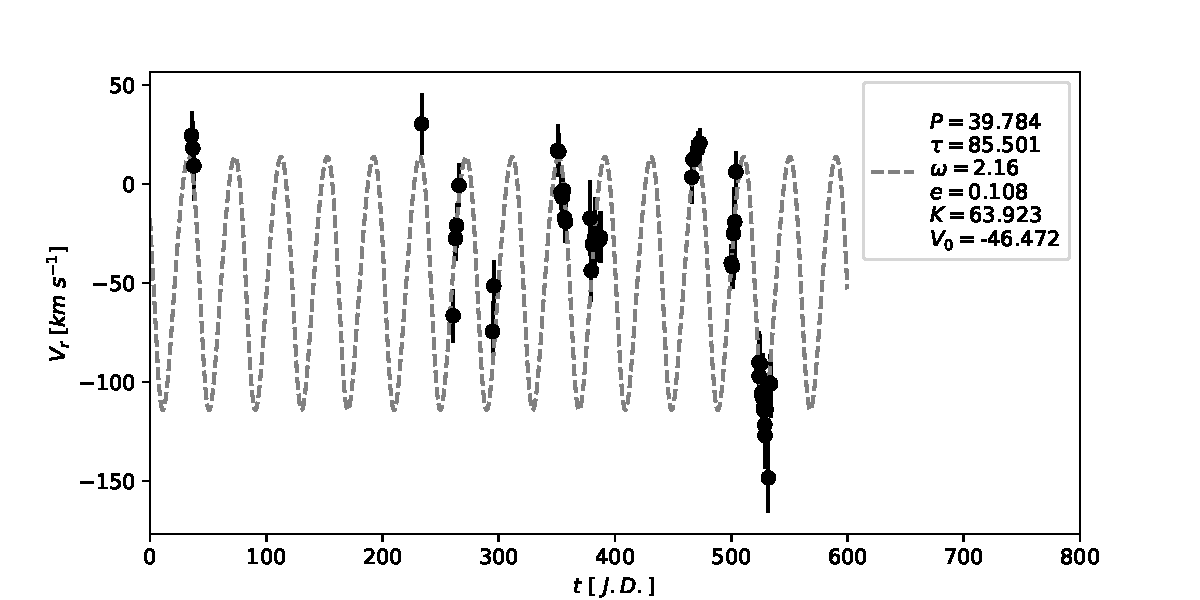
\includegraphics[scale=0.8]{imgs/optimisation/rho_CBr/chosen.pdf}
	\caption{Observations et prédiction pour le vecteur solution $v^2_{sol}$ du tableau \ref{tab:optimisation}}
	\label{fig:opti_finale}
\end{figure}

Au final, la distance paramétrique entres les solutions offertes à la table \ref{tab:optimisation} demeure faible; on suppose que l'ensemble des solutions offertes se retrouvent toutes près du même extrêmum, dans quel cas la moyenne des solutions est un meilleur estimateur de la solution optimale. On utilise donc la moyenne de chaque paramètre pour former un vecteur solution final. On caractérise l'erreur sur ce $v^f_{sol}$ à l'aide des écart-types proposés au même tableau. On bâtit un intervalle de confiance à l'aide des propriétés des lois normales; on choisit un erreur égale à $2 \sigma$ pour construire un intervalle de confiance qui inclut $\approx 95\%$ de nos données. Selon ces hypothèse, on obtient $v^f_{sol} = (39.80\pm0.04, 85\pm50, 2.1\pm0.4, 0.110\pm0.005, 63.9\pm0.6, -47\pm1)$.

\pagebreak

\section*{Conclusion}

En implémentant une variété d'algorithmes basés sur différents types de mutations, il a été possible d'explorer et de comparer les algorithme évolutifs. On conclut que, parmi les stratégies explorées, celle basée sur l'objectif possède la meilleure performance générale. Par contre, $2$ autres types de mutations génèrent régulièrement des vecteurs solutions $v_{sol}$ de haute qualité, soient les mutations standards et les mutations non-uniformes. Une seule stratégie demeure systématiquement moins performante que les autres, soit la stratégie basée sur la distance. Au final, la stratégie employée pour l'optimisation des paramètres $P$, $\tau$, $\omega$, $e$, $K$, et $V_0$ produit des $v_{sol}$ qui sont près les uns les autres en termes de distance paramétrique. On estime alors que ces solutions décrivent toutes le même maximum, qui se situe au point $v^f_{sol} = (39.80\pm0.04, 85\pm50, 2.1\pm0.4, 0.110\pm0.005, 63.9\pm0.6, -47\pm1)$ de l'espace paramétrique.\par
Au final, il demeure difficile de déterminer si $v^f_{sol}$ est réellement un maximum global. Trouverait-on une meilleur solution si on continuait l'exploration? Notre algorithme est-il biaisé dans ses choix de solutions? Bref, il ne s'agit pas de nouvelles questions dans le cadre de l'analyse numérique. Par contre, on peut tout de même se contenter d'une performance accrue et incomparable à celle de procédés itératifs plus simples qui convergent vers l'extremum local le plus près. Avec une telle capacité d'exploration et d'optimisation, il serait intéressant de comparer l'optimisation d'un réseau neuronal par rétropropagation conventionnelle et par évolution adaptive. Les algorithmes évolutifs sont-ils une solution pertinente et réalisable à un problème qui demande déjà beaucoup de ressource de calculs?


\pagebreak

\section{Annexe}

\begin{figure}[H]
	\begin{subfigure}{0.45\linewidth}
		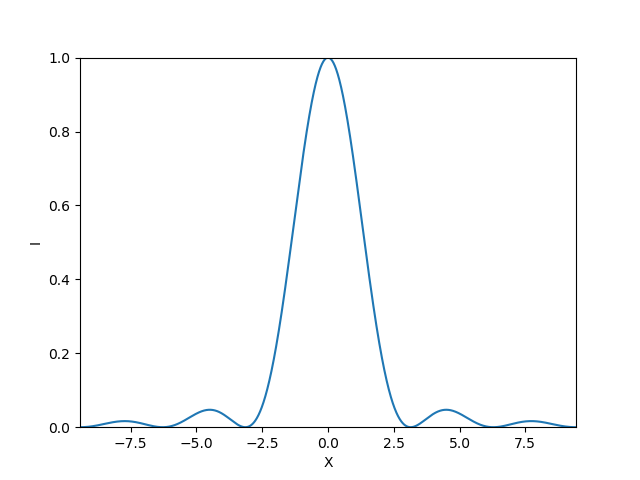
\includegraphics[scale=0.4]{imgs/diff.png}
		\caption{Problème de diffraction 1D. Intensité en fonction de la position.}
		\label{key}
	\end{subfigure}
	\hspace{0.5cm}
	\begin{subfigure}{0.45\linewidth}
		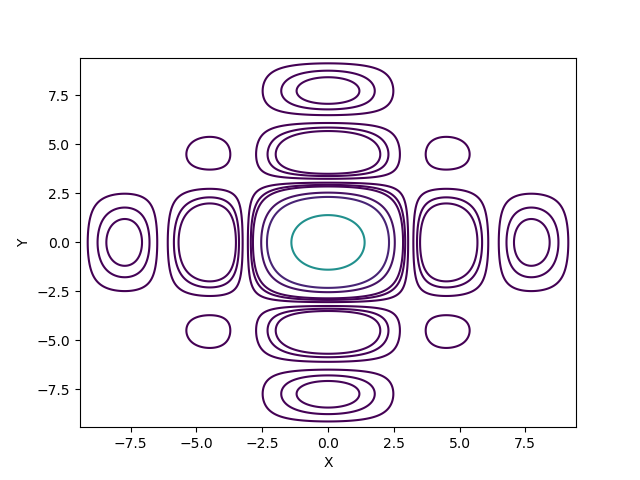
\includegraphics[scale=0.4]{imgs/contour_diffraction.png}
		\caption{Problème de diffraction 2D. Les isocontours prennent une valeur de $[0.001, 0.005, 0.01, 0.05, 0.1, 0.5]$.}
		\label{key}
	\end{subfigure}
	\caption{}
	\label{fig:diffraction}
\end{figure}

\begin{figure}[H]
	\centering
	\begin{subfigure}{.46\linewidth}
		\centering
		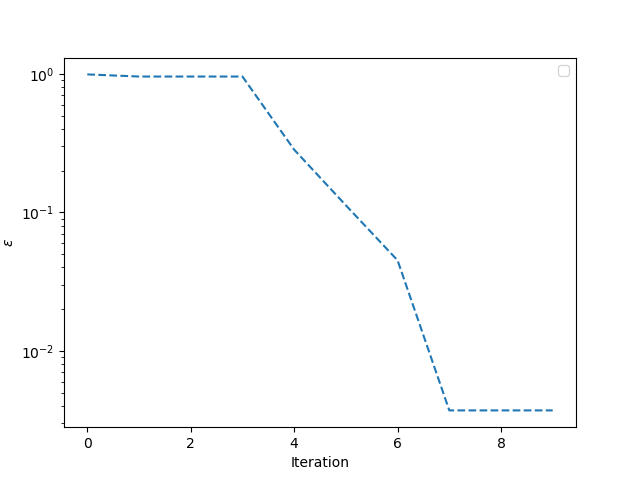
\includegraphics[scale=0.46]{imgs/validation/validation.png}
		\caption{Erreur de la simulation décrite à la figure \ref{fig:diffraction_instant}. }
	\end{subfigure}
	\hspace{0.5cm}
	\begin{subfigure}{.46\linewidth}
		\centering
		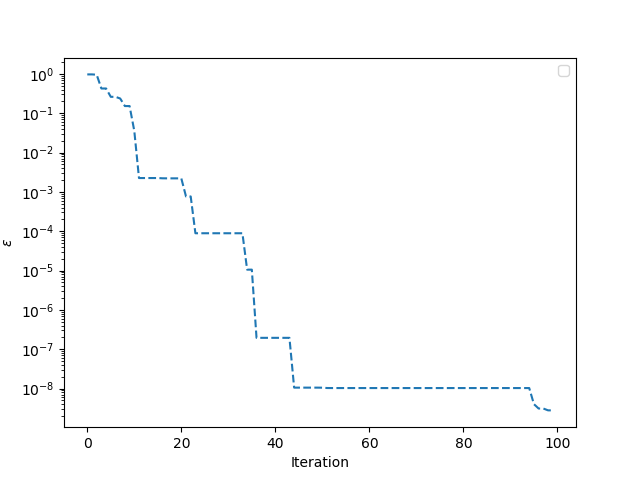
\includegraphics[scale=0.46]{imgs/validation/validation_log.png}
		\caption{Erreur d'une simulation avec les même hyperparamètres que la simulation décrite à la figure \ref{fig:diffraction_instant}, mais qui se poursuit jusqu'à 100 générations.}
	\end{subfigure}
	\caption{}
	\label{fig:diffraction_error}
\end{figure}

\begin{figure}[H]
	\centering
	\foreach \x in {0, 1, ..., 8}{
		\begin{subfigure}{.32\linewidth}
			\centering
			\includegraphics[scale=0.34]{imgs/validation/evolve\x.png}
			\caption{t = \x}
		\end{subfigure}
	}
	\caption{Instantannées des 9 premières étapes d'une simulation à $N=10$, $p_m=0.1$, $p_c=0.8$ et $p_s=0.2$. On remarque que la meilleur solution se situe initialement près d'un maximum local. L'algorithme converge vers un meilleur maximum local dès la première étape. À l'étape 4, on converge vers le maximum global. L'élitisme nous garantie de ne pas s'échapper une fois l'obejctif atteint.}
	\label{fig:diffraction_instant}
\end{figure}



\begin{figure}[H]
	\centering
	\begin{subfigure}{.9\linewidth}
		\centering
		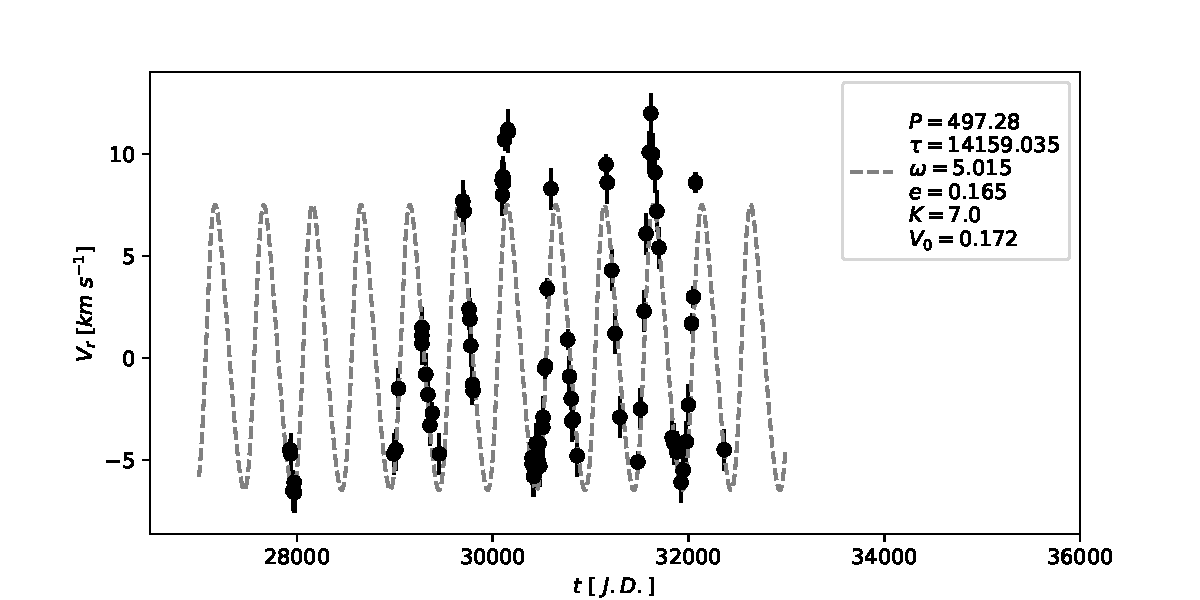
\includegraphics[scale=0.7]{imgs/nbootis/100.pdf}
		\caption{}
	\end{subfigure}
	\begin{subfigure}{.9\linewidth}
		\centering
		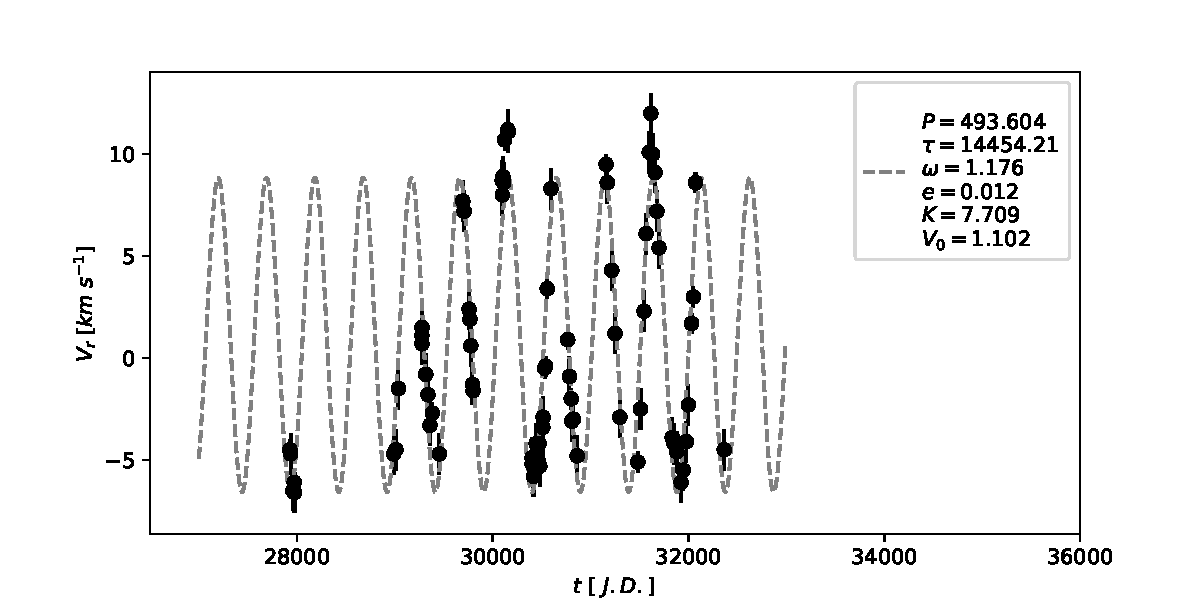
\includegraphics[scale=0.7]{imgs/nbootis/250.pdf}
		\caption{}
	\end{subfigure}
	\begin{subfigure}{.9\linewidth}
		\centering
		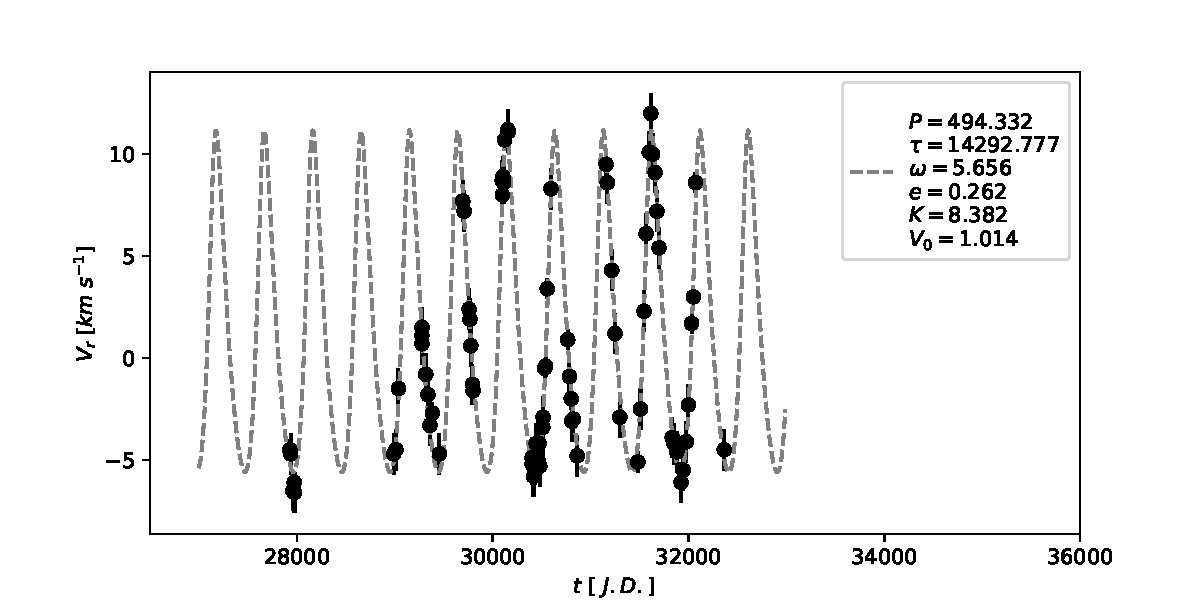
\includegraphics[scale=0.7]{imgs/nbootis/500.pdf}
		\caption{}
	\end{subfigure}
	\caption{Montre trois étapes de l'optimisation du modèle décrivant l'orbite de $\rho CrB$, soit à 100, 250 et 500 générations. On remarque la convergence vers la solution connue.} 
	\label{fig:convergence_orbite}
\end{figure}

\begin{figure}[H]
	\centering
	\foreach \x in {imgs/parameters/N/error_n2.pdf, imgs/parameters/p_m/error_p_m3.pdf, imgs/parameters/p_s/error_p_s2.pdf, imgs/parameters/p_c/error_p_c2.pdf}{
		\begin{subfigure}{.45\linewidth}
			\centering
			\includegraphics[scale=0.45]{\x}
			\caption{}
		\end{subfigure}
	}
	\caption{Trois simulations sont lancées pendant 1000 générations afin de comparer l'effet des hyperparamètres. La figure $a$ montre l'effet de la taille de la population, la figure $b$ montre l'effet de la probabilité de mutation, tandis que la figure $c$ montre l'effet de la pression sélective et la figure $d$, la probabilité de croisement.}
	\label{fig:parametres}
\end{figure}

\section{Bibliographie}\label{sec:bibliographie}
\begin{thebibliography}{l}
	\bibitem{notes_cours} 
	\textsc{Charbonneau}, P., Recueil de notes, Modélisation numérique en physique, Département de Physique, Université de Montréal, Janvier 2019
	
	\bibitem{notes_cours_phy1234} 
	\textsc{Charbonneau}, P., \textsc{Lafrenière}, D., Recueil de notes, Introduction à la physique numérique, Département de Physique, Université de Montréal, Automne 2016
	
	\bibitem{github}
	\textsc{Pfleiderer}, E., Dépôt GitHub,\\ https://github.com/EricPfleiderer/Portfolio/tree/master/PHY3075/PROJET5
	
	\bibitem{neurodim}
	\textsc{www.neurodimension.com},\\ http://www.neurodimension.com/genetic/documentation/OptiGenLibraryDotNet/GeneticServer/Non-Uniform\_Mutation.htm
	
	\bibitem{diro}
	\textsc{Charbonneau}, P., http://www.astro.umontreal.ca/~paulchar/phy3075/phy3075.html
\end{thebibliography}


\end{document}